\documentclass[a4paper,12pt]{article}   % papír A4, písmo 12 bodu
\usepackage[utf8x]{inputenc}            %kodovaní UTF-8
\usepackage{ucs}                        %kodovani unicode
\usepackage[czech]{babel}               %podpora cestiny
\usepackage[T1]{fontenc}                %pouzij variantu pisma T1 (hacky, carky)
\usepackage[left=2.5cm,right=1.5cm,top=2.5cm,bottom=2.5cm]{geometry} %okraje stranky
\usepackage{amsmath,amsfonts,amssymb}   %podpora matematiky
\usepackage{gensymb,marvosym}           %symboly celsius (\celsius) apod.
%\usepackage{mathptmx}                   %font Times New Roman s~podporou matematiky
\usepackage{times}                      %font Times New Roman (matematika pismem Computer Modern) 
\usepackage{parskip}                    %mezera mezi odstavci
%\usepackage[document]{ragged2e}         %text zarovany vlevo
\usepackage[none]{hyphenat} \sloppy     %slova nedelit a~nepretekat
\usepackage{titlesec}
\setcounter{secnumdepth}{4}
\clubpenalty 10000                      %kontrolovat sirotky
\widowpenalty 10000                     %kontrolovat vdovy
\usepackage{setspace} \onehalfspacing   %podpora pro zmenu radkovani + radkovani 1,5
\usepackage{enumerate}                  %podpora pro zmenu cislovani
\usepackage{fancyhdr}                   %vlastni zahlavi a~zapati
\usepackage{graphicx}                   %podpora grafiky
\graphicspath{{materialy/}}                   %vychozi adresar s~obrazky
\usepackage{caption}                    %popisky
\usepackage{subcaption}                 %podpopisky
\usepackage{siunitx}
\usepackage{MnSymbol,wasysym}
\usepackage[shortlabels]{enumitem}
\usepackage{amsmath}
\usepackage{lastpage}                   %zjištění poslední stránky \pageref{LastPage}
\usepackage{float}                      
\usepackage{url}
\usepackage[unicode]{hyperref}          %klikaci odkazy v~textu
\usepackage{mhchem}
\usepackage{multirow}
\usepackage{textgreek}
\usepackage{cancel}
\usepackage{halloweenmath}


\titleclass{\subsubsubsection}{straight}[\subsection]
\newcounter{subsubsubsection}[subsubsection]
\renewcommand\thesubsubsubsection{\thesubsubsection.\arabic{subsubsubsection}}
\renewcommand\theparagraph{\thesubsubsubsection.\arabic{paragraph}} % optional, useful if paragraphs are to be numbered


%------------------------ čtvrtá a~pátá úroveň nadpisu ---------------------------

\titleformat{\subsubsubsection}
  {\normalfont\normalsize\bfseries}{\thesubsubsubsection}{1em}{}
\titlespacing*{\subsubsubsection}
{0pt}{3.25ex plus 1ex minus .2ex}{1.5ex plus .2ex}

\makeatletter

\renewcommand\paragraph{\@startsection{paragraph}{5}{\z@}%
  {3.25ex \@plus1ex \@minus.2ex}%
  {-1em}%
  {\normalfont\normalsize\bfseries}}
\renewcommand\subparagraph{\@startsection{subparagraph}{6}{\parindent}%
  {3.25ex \@plus1ex \@minus .2ex}%
  {-1em}%
  {\normalfont\normalsize\bfseries}}
\def\toclevel@subsubsubsection{4}
\def\toclevel@paragraph{5}
\def\toclevel@paragraph{6}
\def\l@subsubsubsection{\@dottedtocline{4}{7em}{4em}}
\def\l@paragraph{\@dottedtocline{5}{10em}{5em}}
\def\l@subparagraph{\@dottedtocline{6}{14em}{6em}}
\makeatother

\setcounter{secnumdepth}{4}
\setcounter{tocdepth}{4}


\setlist[enumerate]{itemsep=0mm}
%_____________________________|___________________________|_____________________________%
%                             |                           |                             %
%-----------------------------| ZDE VYPLNIT UDAJE O PRACI |-----------------------------%
%_____________________________|___________________________|_____________________________%
%                             

\newcommand{\nazev}{Nevyvážený Wheatstoneův můstek - vyhodnocení změny odporu odporového snímače}                                                        %
\newcommand{\jmeno}{Jakub Dvořák}                                                     %
\newcommand{\datum}{21.11.2020}                                                              %
%---------------------------------------------------------------------------------------%


%-----------------------------| POUŽITÁ MAKRA |-----------------------------%

%\newcommand{\zkratka}{ve výsledku se mi napíše tenhle text}
%\newcommand{}{}
%\newcommand{}{}
%\newcommand{}{}
\newcommand{\tsub}[1]{$_\textrm{#1}$}
\newcommand{\texp}[1]{$^\textrm{#1}$}
\newcommand{\tohm}{$\Omega$}
\newcommand{\tmu}{$\mu$}
\newcommand{\var}[2]{$#1_\text{#2}$}
\newcommand{\larrow}{$\leftarrow~$}
\newcommand{\rarrow}{$\rightarrow~$}
\newcommand{\rrarrow}{$\longrightarrow~$}
\newcommand{\llarrow}{$\longleftarrow~$}


%_______________________________________________________________________________________%
%_______________________________________________________________________________________%


%----------------------------------- KONEC PREAMBULE -----------------------------------%






%-------------------------------------- DOKUMENT --------------------------------------%
%______________________________________________________________________________________%
\begin{document} %%%%%%%%%%%%%%%%%%%%%%%%%%%%%%%%%%%%%%%%%%%%%%%%%%%%%%%%%%%%%%%%%%%%%%%

\setcounter{page}{0} %cislo strany
\pagestyle{empty} %stranku necislovat

%prostredi pro grafy a~schemata \begin{graf} \begin{schema}
\newfloat{schema}{htbp}{schema}\floatname{schema}{Schéma}
\newfloat{graf}{htbp}{graf}\floatname{graf}{Graf}

\begin{titlepage}
    \begin{center}
        \vspace*{1cm}
            
        \Huge
        \textbf{\nazev}
            
        \vspace{0.5cm}
        \LARGE
            
        \vspace{1.5cm}
            
        \textbf{\jmeno}
            
        \vfill
            
        \vspace{0.8cm}
            
        \Large
            
        \datum\\
        \vspace*{.5cm}
        
\includegraphics[width=.4\textwidth]{logo-cvut-fee.png}\\
    \end{center}
\end{titlepage}

% --- definice zapati a~cislovani ---
\newpage 
\pagestyle{fancy}                                       %vlastni zahlavi/zapati
\renewcommand{\headrulewidth}{0pt}                      %bez linky v~zahlavi
\renewcommand{\footrulewidth}{.5pt}                    %linka v~zapati - optional
\lhead{}       \chead{} \rhead{\nazev}                        %pole zahlavi (prazdna)
\lfoot{\jmeno} \cfoot{} \rfoot{\thepage}   %pole zapati


%------------------------------------ VLASTNÍ TEXT ------------------------------------%



\section{Úkol měření}
\label{chap:ukol}
\begin{enumerate}
    \item 
      \begin{enumerate}[label=\alph*)]
        \item  Zapojte převodník R \rarrow U s operačním zesilovačem podle schématu na obr. 1 (\var{U}{r} = 10 V, \var{R}{N1} = 10 k\tohm) a změřte závislost odporu snímače na jeho úhlové      výchylce \var{\alpha} v rozsahu \var{\alpha}{} = 0 až 180° po 15° (klidové poloze snímače \var{\alpha} = 90° odpovídá hodnota odporu \var{R}{0}, tj. \var{\Delta}{}\var{R}{}~=~0).
        \item Odporový snímač zapojte do Wheatstoneova můstku napájeného ze zdroje napětí \var{U}{AC} = 5~V (obr. 2). Můstek vyvažte odporovou dekádou \var{R}{D} pro hodnotu \var{\alpha}{} = 90° a změřte závislost \var{f}{MN} výstupního napětí \var{U}{BD} na změně úhlu \textalpha, tj. na změně odporu ∆R (pro stejné hodnoty \textalpha\ jako v bodě 1). Odvoďte teoretický vztah pro toto napětí, tj.
      \end{enumerate}
      \begin{equation}
        U_{BD} = f_{MN}(\Delta R)=\frac{U_{AC}}{4}\frac{\frac{\Delta R}{R_0}}{1+\frac{\Delta R}{2R_0}}
      \end{equation}
      \item Odporový snímač zapojte do Wheatstoneova můstku napájeného ze zdroje proudu \var{I}{} = 2,5 mA. Zdroj proudu realizujte pomocí operačního zesilovače (obr. 3). Můstek opět vyvažte odporovou dekádou \var{R}{D} pro hodnotu \textalpha\ = 90° a změřte závislost fMP výstupního napětí \var{U}{BD} na změně úhlu \textalpha, tj. na změně odporu \var{\Delta}{} R (pro stejné hodnoty \textalpha\ jako v bodě 1). Odvoďte teoretický vztah pro toto napětí, tj.
      \begin{equation}
        U_{BD} = f_{MN}(\Delta R)=\frac{I}{4}\frac{\Delta R}{1+\frac{\Delta R}{4R_0}}
      \end{equation}
      \item Podle schématu na obr. 4 zapojte tzv. „linearizovaný můstek" (velikost napájecího napětí volte \var{U}{Z} = 2,5 V). Můstek vyvažte odporovou dekádou RD pro hodnotu \textalpha\ = 90° a změřte závislost \var{U}{2} = \var{f}{LM} výstupního napětí \var{U}{2} na změně úhlu \textalpha, tj. na změně odporu \var{\Delta}{}R (pro stejné hodnoty úhlu \textalpha jako v předešlých bodech). Odvoďte teoretický vztah pro toto napětí, tj.
      \begin{equation}
        U_2 = f_{LM}(\Delta R) = -\frac{\Delta R}{2R_0}U_Z
      \end{equation}
      \item Do společného grafu vyneste odchylky hodnot naměřených dle bodů 2, 3 a 4 od lineárního průběhu. Směrnici přímky, od které budete určovat odchylky od linearity, stanovte z koncových bodů naměřené závislosti \var{f}{LM}\var{(\Delta R)}{} (tedy pro \textalpha\ = 0 a \textalpha\ = 180°). Pokud se absolutní hodnoty napětí v koncových bodech liší, nahraďte je aritmetickým průměrem těchto absolutních hodnot (spojnice \var{U'}{2} = \var{f'}{LM}(\var{\Delta}{}R) takto upravených koncových bodů prochází počátkem souřadnic [\var{\Delta}{}R, \var{U}{2}]). Odchylky závislostí \var{f}{MN}(\var{\Delta}{}R), \var{f}{MP}(\var{\Delta}{}R) a \var{f}{LM}(\var{\Delta}{}R) od linearity určete jako odchylky těchto závislostí od přímky \var{U'}{2} = \var{f'}{LM}(\var{\Delta}{}R). To lze udělat proto, že pro měření dle bodů 2, 3 a 4 jsou v zadáních zvoleny hodnoty napájecích napětí (resp. proudu) tak, aby směrnice všech závislostí v počátku byly zhruba stejné.
\end{enumerate}


\section{Schéma zapojení}
\label{chap:schema_zapojeni}
\begin{figure}[htbp]
  \centering
  \begin{minipage}{.4\textwidth}
    \captionsetup{width=\textwidth}
    \centering
    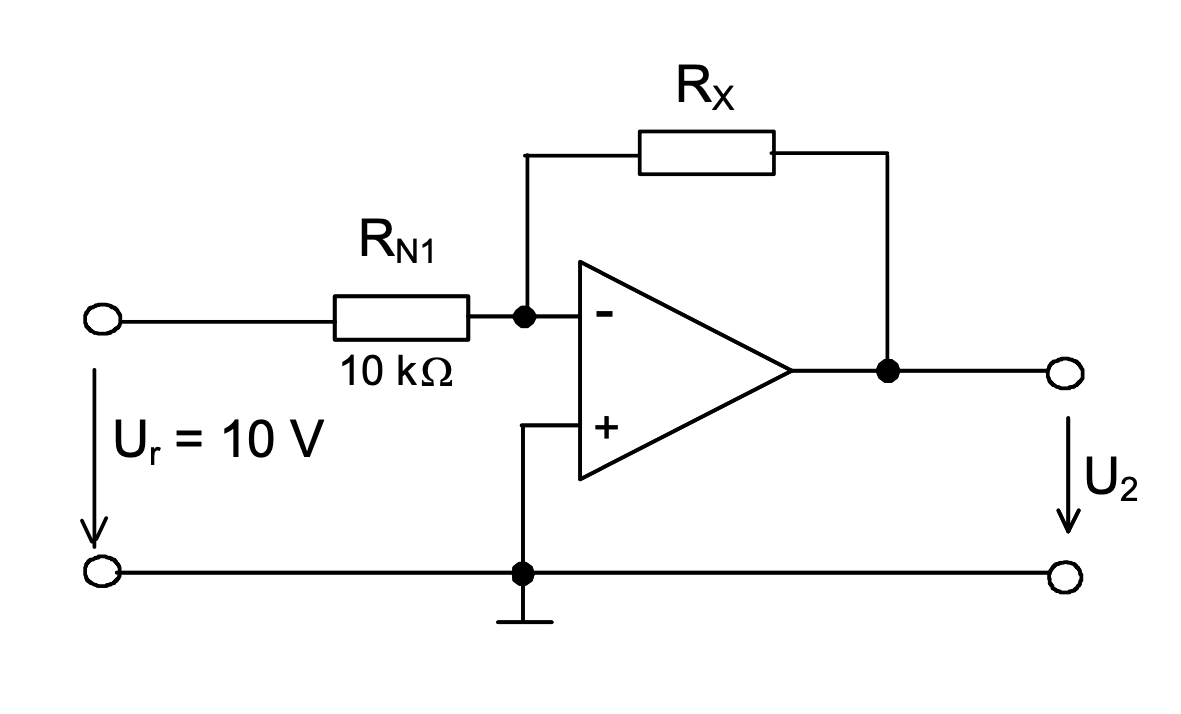
\includegraphics[width=\textwidth]{ru.png}
    \caption{Schéma zapojení pro převodník R $\rightarrow$ U}
    \label{fig:ru} 
  \end{minipage}
  \begin{minipage}{.4\textwidth}
    \captionsetup{width=.8\textwidth}
    \centering
    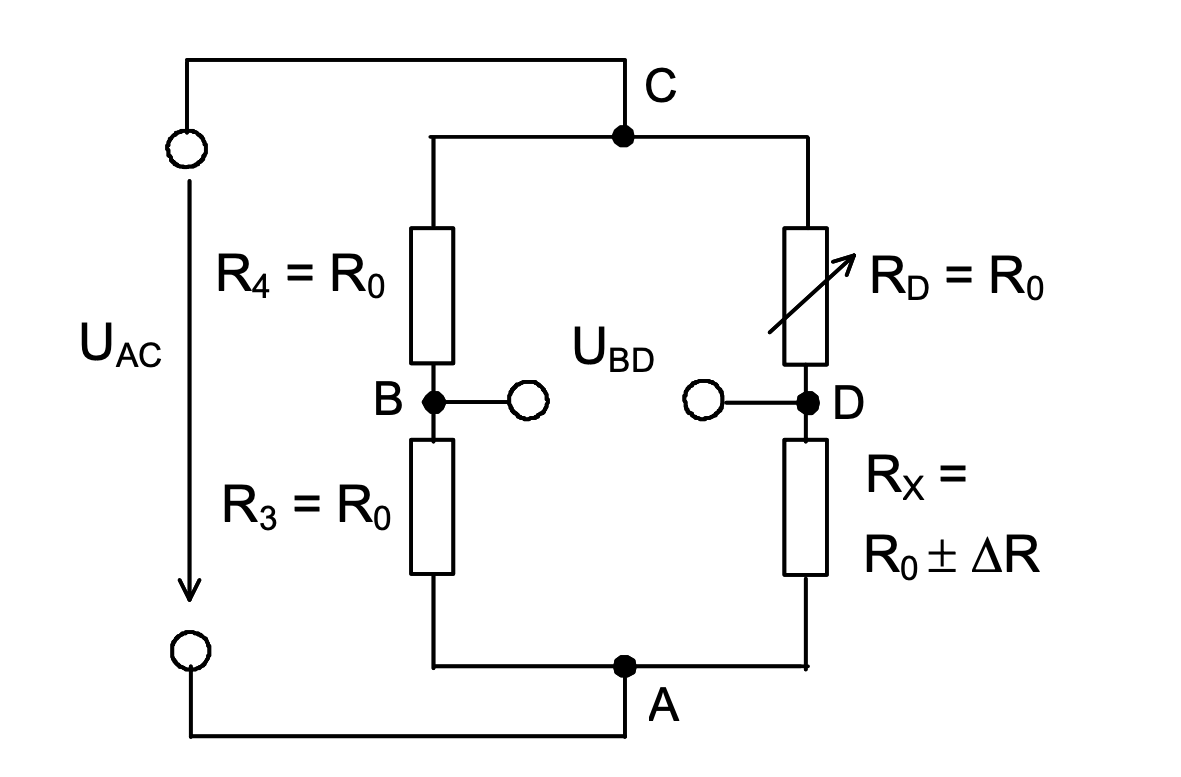
\includegraphics[width=\textwidth]{whu.png}
    \caption{Wheatstoneův můstek napájený ze zdroje napětí}
    \label{fig:whu}
  \end{minipage}
\end{figure}
\begin{figure}[h!]
  \centering
  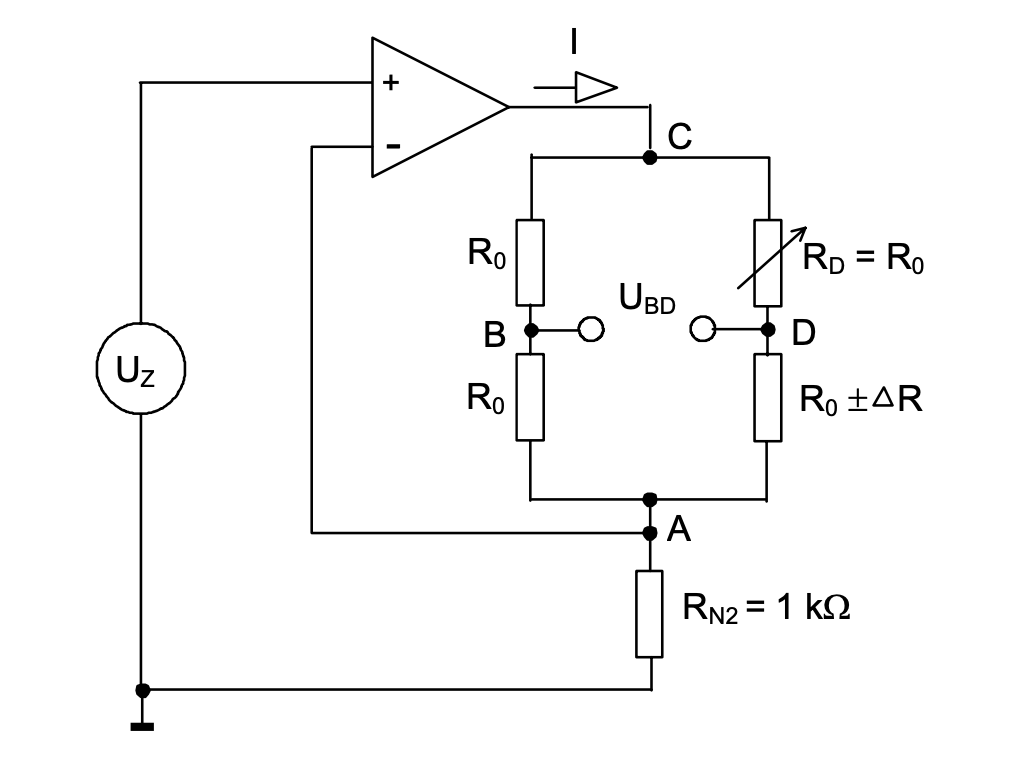
\includegraphics[width=.5\textwidth]{whi.png}
  \caption{Wheatstoneův můstek napájený ze zdroje proudu}
  \label{fig:whi}
\end{figure}
\newpage



\section{Seznam použitých přístrojů}
\label{chap:seznam_pristroju}
\begin{table}
  \begin{tabular}{ll}
    Př 1 & - přípravek s operačním zesilovačem\\
    Př 2 & - přípravek s dvojicí rezistorů\\
    Př 3 & - přípravek s odporovým snímačem úhlu\\
    \var{\text{Z}}{1} & - napájecí zdroj operačního zesilovače\\
    \var{\text{Z}}{1} & - číslicově řízený zdroj ss napětí \var{\text{U}}{Z}\\
    ČV & - číslicový voltmetr typ: Agilent 34401A\\
    \var{\text{R}}{N1} & - rezistor 10~k\tohm\\
    \var{\text{R}}{N1} & - rezistor 1~k\tohm\\
    \var{\text{R}}{D} & - odporová dekáda
  \end{tabular}
\end{table}


\section{Teoretický úvod}
\label{chap:teoreticky_uvod}
Pro zapojení podle obrázku \ref{fig:ru} platí
\begin{equation*}
  U_\text{2} = -U_\text{r}\frac{U_\text{x}}{R_\text{N1}}.
\end{equation*}
Pro velikost měřeného odporu tedy platí
\begin{equation}
  U_\text{x}=-R_\text{N1} \frac{U_\text{2}}{R_\text{r}}.
\end{equation}

Nevyvážený Wheatstoneův můstek se většinou využívá při měření neelektrických veličin, které jsou různými senzory převáděny na elektrický odpor.

\section{Naměřené hodnoty}
\label{chap:namerene_hodnoty}



\section{Zpracování naměřených hodnot}
\label{chap:zpracovani_hodnot}

Hodnoty z kapitoly \ref{chap:ukol} jsou zaneseny v tabulce \ref{tab:master}.
\begin{table}[]
  \hspace*{-1.5cm}
  \begin{tabular}{|r|r|r||r|r||r|r||r|r||r|}\hline
  $\alpha$   (\textdegree) & $R_X$ (\tohm ) & $\Delta R$ (\tohm ) & $U$   (mV) & $\Delta U$ (mV) & $U$   (mV) & $\Delta U$ (mV) & $U$   (mV) & $\Delta U$ (mV) & Lin. (mV) \\\hline\hline
  180                      & 2080,5       & -315,1             & -204,52              & -7,59                     & -198,82              & -13,29                    & -222,70             & 10,59                     & -212,11    \\\hline
  170                      & 2041,5       & -276,1             & -181,16              & 11,47                     & -175,15              & 5,46                      & -195,67             & 25,98                     & -169,69    \\\hline
  150                      & 1976,8       & -211,4             & -141,08              & 13,82                     & -135,20              & 7,93                      & -149,46             & 22,20                     & -127,27    \\\hline
  130                      & 1905,1       & -139,7             & -94,34               & 9,49                      & -89,81               & 4,96                      & -98,13              & 13,28                     & -84,84     \\\hline
  110                      & 1835,7       & -70,3              & -48,12               & 5,69                      & -45,14               & 2,71                      & -48,95              & 6,53                      & -42,42     \\\hline
  90                       & 1765,4       & 0,00               & 0,00                 & 0,00                      & 0,00                 & 0,00                      & 0,00                & 0,00                      & 0,00       \\\hline
  70                       & 1696,8       & 68,6               & 49,04                & -6,62                     & 45,53                & -3,11                     & 48,47               & -6,05                     & 42,42      \\\hline
  50                       & 1632,5       & 132,9              & 97,65                & -12,80                    & 88,93                & -4,09                     & 93,95               & -9,10                     & 84,84      \\\hline
  30                       & 1564,5       & 200,9              & 150,57               & -23,31                    & 135,68               & -8,42                     & 142,03              & -14,77                    & 127,27     \\\hline
  10                       & 1504,8       & 260,6              & 198,97               & -29,28                    & 177,51               & -7,82                     & 184,28              & -14,59                    & 169,69     \\\hline
  00                        & 1466,7       & 298,7              & 230,76               & -18,65                    & 204,62               & 7,49                      & 211,23              & 0,88                      & 212,11    \\\hline
  \end{tabular}
  \caption{Vypočtené hodnoty rozdílů napětí od lineární funkce}
  \label{tab:master}
\end{table}


Jednotlivé rozdíly napětí od lineární funkce jsou zakresleny v grafu.
\begin{graf}
  \centering
  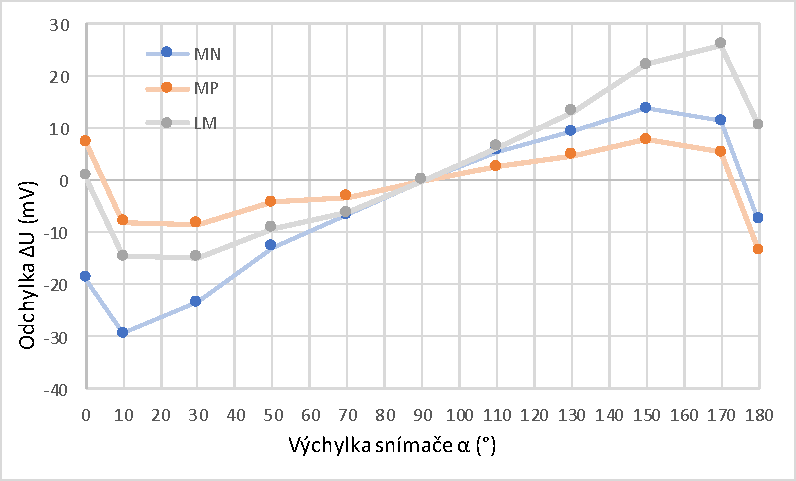
\includegraphics[width=\textwidth]{graf1.pdf}
  \caption{Závislost rozdílu změny napětí od lineární funkce na výchylce snímače}
  \label{gr:delta}
\end{graf}


\subsection{Odvození vztahů}
\begin{equation}
  \begin{split}
    U_\text{BD} &= U_\text{B} - U_\text{D} = \left(U_\text{AC}\frac{R_0}{2R_0}\right)-\left(U_\text{AC}\frac{R_0+\Delta R}{2R_0+\Delta R}\right)\\
    U_\text{BD} &= U_\text{AC}\left(\frac{1}{2}-\frac{R_0}{2R_0+\Delta R}\right) = U_\text{AC}\frac{2R_0+\Delta R -2(R_0+\Delta R)}{4R_0 + 2\Delta R} = -U_\text{AC}\frac{\Delta R}{2(2R_0+\Delta R)}\\
    U_\text{BD} &= -\frac{U_\text{AC}}{4}\cdot\frac{\frac{\Delta R}{R_0}}{1+\frac{\Delta R}{2R_0}}\\
  \end{split}
\end{equation}

Pro odvození vztahu pro proudový zdroj budeme vycházet z proudového děliče:
\begin{equation}
  \frac{I_\text{B}}{I} = \frac{\frac{U}{2R_0}}{U\frac{4R_0+\Delta R}{2R_0(2R_0 + \Delta R)}} = \frac{\cancel{U}}{\cancel{2R_0}}\cdot \frac{\frac{\cancel{2R_0}(2R_0 + \Delta R)}{{4R_0+\Delta R}}}{\cancel{U}} = \frac{2R_0+\Delta R}{4R_0 + \Delta R} \rightarrow I_\text{B} = {{\frac{2R_0+\Delta R}{4R_0 + \Delta R} \cdot I}}
\end{equation}
\begin{equation}
  I_\text{D} = I - I_\text{B} = I\left(1-\frac{2R_0+\Delta R}{4R_0 + \Delta R}\right) = {\frac{2R_0}{4R_0+\Delta R}}
\end{equation}
\begin{equation}
  U_\text{BD} = R_0 I_\text{B} -\left(R_0+\Delta R\right)\cdot I_\text{D} = -I\frac{R_0+\Delta R}{4R_0 + \Delta R} = \underline{\underline{-\frac{I}{4}\cdot\Delta \frac{1}{1+\frac{\Delta R}{4R_0}}}}
\end{equation}


\section{Závěrečné vyhodnocení}
Jak je vidět z grafu \ref{gr:delta}, tak nejvíce přesná metoda je můstek napájený ze zdroje proudu. Nicméně v praxi je nejpřesnější metoda linearizovaného můstku. Tato chyba mohla vzniknout například nepřesným určováním polohy úhlu ručičky. Další zdroj nepřesnosti mohl být nesprávné vyvážení můstku na začátku měření.

%--- LITERATURA a~ZDROJE (povinne) ---
\clearpage
\renewcommand{\refname}{Seznam použité literatury a~zdrojů informací} 
%\section*{Seznam použité literatury a~zdrojů informací}
\phantomsection %pridej odkaz do PDF zalozek
\addcontentsline{toc}{section}{Seznam použité literatury a~zdrojů informací}

\begin{thebibliography}{99}

%----------------------------------------------------
\subsection*{Seznam použitých internetových zdrojů}
    \bibitem{navod} Návod k~laboratorní úloze
    
\end{thebibliography}

\end{document}